% LREC-COLING 2026 Submission (draft scaffold)
% NOTE: This LaTeX file is an ENGLISH outline to be finalized after
% verifying the Ukrainian MD source-of-truth:
%   Experiments/dyspnea_crf_eval/LREC2026_Paper/System_Description_Paper_UA.md

\documentclass[10pt, a4paper]{article}
\usepackage[review]{lrec2026}
\usepackage[utf8]{inputenc}
\usepackage{tikz}
\usetikzlibrary{arrows.meta, positioning}


\title{MedGemma StructCore: Schema-Guided Condensation\\and Deterministic Compilation for CRF Filling\\(CL4Health 2026 System Description)}

\name{Anonymous Submission}
\address{Affiliation \\
         Address \\
         email@example.com}

\abstract{
Automatically filling Case Report Forms (CRFs) from clinical notes is challenging due to noisy language, strict output contracts, and the high cost of false positives. We describe our CL4Health 2026 submission for Dyspnea CRF filling (134 items) using a \textit{contract-driven} two-stage design grounded in \textit{Schema-Guided Reasoning (SGR)}. The key task property is extreme sparsity: many fields are \texttt{unknown}, and official scoring penalizes empty values and unsupported predictions. We therefore shift from a single-step ``LLM predicts 134 fields'' approach to a decomposition where (i) Stage~1 produces a stable SGR-style JSON summary with exactly 9 domain keys; and (ii) Stage~2 is a fully deterministic compiler that parses the Stage~1 summary, canonicalizes item names (optionally using a UMLS alias map with 134/134 coverage), normalizes predictions to the official controlled vocabulary, and expands the output into the required 134-item submission format with missing values set to \texttt{unknown}. Preliminary results on the official train split (N=10) highlight the importance of Stage~1 recall and evidence-gated post-filters for high-FP items.
\\ \newline \Keywords{clinical NLP, information extraction, LLM systems, controlled vocabulary, reproducibility, edge AI}}

\begin{document}
\maketitleabstract

\section{Introduction}
The CL4Health 2026 CRF filling shared task requires mapping unstructured clinical notes to a strict 134-item Dyspnea CRF. In practice, end-to-end LLM extraction often fails either due to output format drift (invalid JSON/submission structure) or due to unsupported ``hallucinated'' fills that increase false positives (FP). Our design goal is to separate (a) clinical information condensation from (b) contract enforcement and controlled-vocabulary normalization, while using SGR to make the intermediate representation stable and machine-checkable.

\paragraph{SGR in brief.}
Schema-Guided Reasoning (SGR) \cite{abdullin2026sgr} is an architectural pattern that constrains an LLM to produce typed, schema-conformant outputs (via structured output or constrained decoding \cite{dong2024xgrammar}), turning domain knowledge into executable data contracts. This reduces variability and improves reliability compared to free-form text prompting. In our system, Stage~1 uses an SGR-style schema with three key patterns to produce a stable 9-key domain summary:
\begin{itemize}
    \item \textbf{Cascade (Domain Scaffold):} The LLM follows a fixed sequence of 9 clinical domains (Demographics, Vitals, Labs, Problems, Symptoms, Medications, Procedures, Utilization, Disposition) to ensure uniform coverage.
    \item \textbf{Cycle (Checklists):} The prompt enforces implicit checklists (e.g., forcing examination of 28 specific CRF problems and critical vitals).
    \item \textbf{Routing (Vocabulary):} While Stage~1 emits unconstrained strings, Stage~2 deterministically routes predictions into the 13 required vocabulary categories.
\end{itemize}
Stage~2 then deterministically compiles this summary into the official CRF submission format.

\section{Task and Data}
We use the official Hugging Face datasets (\texttt{NLP-FBK/dyspnea-crf-*}) and, for teacher generation, the in-domain unannotated notes set (\texttt{NLP-FBK/dyspnea-clinical-notes}). A key discovery is sparsity: many items are \texttt{unknown}, and \texttt{unknown} must be treated as a valid semantic class. The official submission is JSONL with 134 \texttt{item/prediction} pairs per document; missing/blank values are not acceptable in practice.

\paragraph{Contract-driven dataset parsing.}
We align our pipeline contracts directly to the dataset schema: (i) the ordered list of 134 items is inferred from the official record (\texttt{annotations[*].item} or \texttt{expected\_crf\_items}) and reused end-to-end; (ii) document identifiers are normalized to a plain id (prefix before the first underscore) for internal artifacts and reference alignment, and suffixed with the language tag (\texttt{\_en}/\texttt{\_it}) only for final submissions; (iii) intermediate representations can be sparse, but the final builder always expands to all 134 items and fills missing values with \texttt{unknown}.

\section{System Overview}
Our pipeline is:
\begin{quote}
\texttt{Clinical Note} $\rightarrow$ \texttt{Stage1: SGR-style JSON} $\rightarrow$ \texttt{Stage2: deterministic compile} $\rightarrow$ \texttt{Submission.jsonl}
\end{quote}

\begin{figure}[h]
\centering
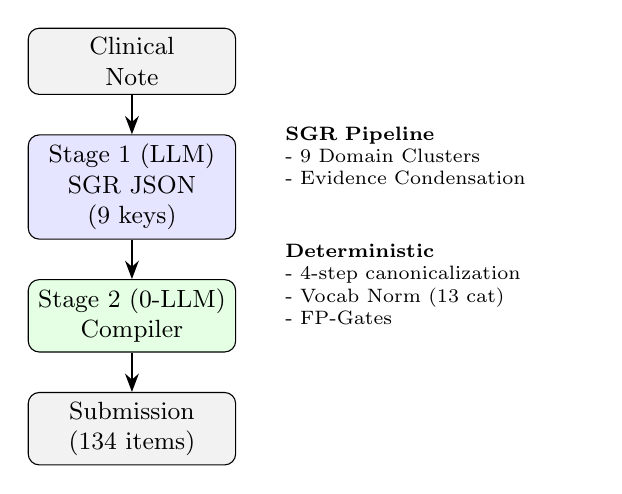
\begin{tikzpicture}[
    node distance=0.5cm and -0.2cm,
    box/.style={draw, rounded corners, align=center, fill=gray!10, text width=2.4cm, font=\small},
    arrow/.style={-{Stealth}, thick}
]
\node[box] (note) {Clinical\\Note};
\node[box, below=of note, fill=blue!10] (stage1) {Stage 1 (LLM)\\SGR JSON\\(9 keys)};
\node[box, below=of stage1, fill=green!10] (stage2) {Stage 2 (0-LLM)\\Compiler};
\node[box, below=of stage2] (crf) {Submission\\(134 items)};

\draw[arrow] (note) -- (stage1);
\draw[arrow] (stage1) -- (stage2);
\draw[arrow] (stage2) -- (crf);

\node[anchor=west, text width=3.8cm, font=\scriptsize, align=left] at ([xshift=0.5cm, yshift=0.4cm]stage1.east) {\textbf{SGR Pipeline}\\- 9 Domain Clusters\\- Evidence Condensation};
\node[anchor=west, text width=3.8cm, font=\scriptsize, align=left] at ([xshift=0.5cm, yshift=0.4cm]stage2.east) {\textbf{Deterministic}\\- 4-step canonicalization\\- Vocab Norm (13 cat)\\- FP-Gates};

\end{tikzpicture}
\caption{The MedGemma StructCore Two-Stage Pipeline Architecture}
\label{fig:pipeline}
\end{figure}

\subsection{Stage 1: SGR-style JSON Summary (9 keys)}
Stage~1 produces a single JSON object with exactly 9 domain keys:
\texttt{DEMOGRAPHICS, VITALS, LABS, PROBLEMS, SYMPTOMS, MEDICATIONS, PROCEDURES, UTILIZATION, DISPOSITION}.
The summary is designed to be sparse (only evidence-supported facts) and format-stable (JSON parse success). Preliminary stability on train10 shows \texttt{json\_parse\_ok=10/10} and \texttt{thinking\_leak=0/10}.

\subsection{Stage 2: Deterministic Compiler (0-LLM)}
Stage~2 performs no LLM calls. It utilizes a 4-step algorithm:
\begin{enumerate}
    \item \textbf{KV Extraction}: Parses the Stage~1 summary into a normalized key/value string dictionary.
    \item \textbf{Canonicalization}: Canonicalizes field names via exact match, case-folding, and punctuation stripping. Optionally, a UMLS alias map handles complex synonymy.
    \item \textbf{FP-Gates \& Derivation}: Derives high-FN composite items (e.g., deriving \textit{poly-pharmacological therapy} or \textit{antihypertensive therapy} by analyzing the extracted 35 hypertensive and 17 anticoagulant agents from the Stage~1 string). Then it applies strict Regex-based evidence gates to drop unsupported positive predictions for items like \textit{active neoplasia} and \textit{acute coronary syndrome}.
    \item \textbf{Normalization (13 Categories)}: Normalizes strings to the strict controlled vocabulary (binary, AVPU, chronic, resp\_rate, duration limits, numeric bounds) and expands to 134 items (filling \texttt{unknown}).
\end{enumerate}

\subsection{Optional UMLS Alias Mapping}
We curated a UMLS-based alias map for all 134 CRF items (coverage 134/134) and integrated it as an optional pipeline mode to reduce key-name brittleness in model outputs.

\section{Experiments and Preliminary Results}
We report preliminary results on small official subsets for debugging and ablation.

\paragraph{Teacher vs.\ Student Stage~1 (N=10, train split).}
Using a stronger teacher model for Stage~1 (Gemini) with the same deterministic Stage~2 improves macro-F1 but increases FP, motivating stricter evidence-gated filters.

\paragraph{SGR-only end-to-end baseline (N=10, train split).}
Stage~1 (profile=9) $\rightarrow$ Stage~2(det) yields macro-F1 \texttt{0.438431} with \texttt{TP/FP/FN=39/44/39}. This baseline prioritizes format stability and fully deterministic Stage~2 behavior; future work targets Stage~1 recall and FN-first compiler derivations.

\section{Limitations}
The deterministic Stage~2 cannot recover facts missing from Stage~1 summaries; thus overall recall is Stage~1-limited. Additionally, some CRF items require nuanced contextual interpretation that may be lost in short summaries, increasing FN risk. High FP cost requires conservative evidence gating, potentially trading off recall for precision.

\section{Discussion}
\label{sec:discussion}
\subsection{Effectiveness of SGR Patterns}
Applying SGR shifts the burden of structural correctness from prompt engineering to code. By having the LLM emit a stable, 9-key intermediate tree rather than fighting the strict 134-item output length limitations, we achieve 100\% parsing stability even on 4B Edge models without strict grammar tuning.
\subsection{SGR for Edge AI}
This methodology is particularly enabling for Edge (local) deployments. Large state-of-the-art models can handle 134 items easily, but quantized 4B-8B local models lose track of the schema. Our SGR-constrained condensation fits within the reasoning bounds of smaller models, securely delegating the complex vocabulary checks to Python.

\section{Ethical Considerations}
We use publicly available datasets under the organizer terms. We avoid including private clinical data beyond what is distributed by the shared task. When synthetic teacher-generated data is used for training, it should be validated and accompanied by clear documentation of risks and limitations.

\section{Conclusion}
MedGemma StructCore emphasizes contract alignment, format stability, and reproducible post-processing for CRF filling under extreme sparsity. The two-stage design isolates extraction from strict submission enforcement, enabling rapid iteration on Stage~1 recall and controlled-vocabulary grounding without sacrificing deterministic output guarantees.

\section{Bibliographical References}
\label{sec:reference}
\bibliographystyle{lrec2026-natbib}
\bibliography{medgemma_structcore}

\end{document}
